\documentclass[tikz,border=5pt]{standalone}
\usepackage[UTF8]{ctex}
\usepackage{amsmath,amssymb}
\usetikzlibrary{arrows.meta,calc,angles,quotes,decorations.pathmorphing,patterns}
\definecolor{ink}{HTML}{243447}\definecolor{blue}{HTML}{2765A2}
\definecolor{green}{HTML}{3F7D5B}\definecolor{red}{HTML}{B74739}
\tikzset{body/.style={draw=ink,thick},vec/.style={draw=blue,thick,-{Latex}},guide/.style={gray!60,dashed},dim/.style={ink,{Latex}-{Latex}},line cap=round,line join=round}
\begin{document}

\begin{tikzpicture}
\coordinate(L)at(0,0);\coordinate(A)at(2,0);\coordinate(B)at(4,0);
\coordinate(U)at(1,1.732);\coordinate(T)at(2,3.464);\coordinate(V)at(3,1.732);\coordinate(O)at(2,1.1547);
\foreach\from/\to in{L/U,U/T,T/V,V/B,B/A,A/L,O/U,O/V,O/A}{
\draw[body](\from)--(\to);
\path let \p1=($(\to)-(\from)$),\n1={atan2(\y1,\x1)} in
node[draw=ink,fill=white,minimum width=6mm,minimum height=2mm,inner sep=0pt,rotate=\n1]at($(\from)!.5!(\to)$){};
}

\foreach\P in{L,A,B,U,T,V,O}\fill[ink](\P)circle(2pt);
\node[below]at(A){$A$};\node[below right]at(B){$B$};
\node[below]at(2,-.65){各小段电阻均为 $r$};
\end{tikzpicture}
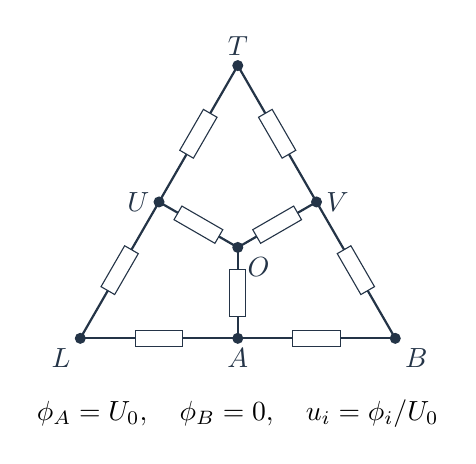
\begin{tikzpicture}
\coordinate(L)at(0,0);\coordinate(A)at(2,0);\coordinate(B)at(4,0);
\coordinate(U)at(1,1.732);\coordinate(T)at(2,3.464);\coordinate(V)at(3,1.732);\coordinate(O)at(2,1.1547);
\foreach\from/\to in{L/U,U/T,T/V,V/B,B/A,A/L,O/U,O/V,O/A}{
\draw[body](\from)--(\to);
\path let \p1=($(\to)-(\from)$),\n1={atan2(\y1,\x1)} in
node[draw=ink,fill=white,minimum width=6mm,minimum height=2mm,inner sep=0pt,rotate=\n1]at($(\from)!.5!(\to)$){};
}
\foreach\P/\pos in{L/below left,A/below,B/below right,U/left,T/above,V/right,O/below right}
\fill[ink](\P)circle(2pt)node[\pos]{$\P$};

\node[below]at(2,-.65){$\phi_A=U_0,\quad\phi_B=0,\quad u_i=\phi_i/U_0$};
\end{tikzpicture}
\begin{tikzpicture}
\coordinate(L)at(0,0);\coordinate(A)at(2,0);\coordinate(B)at(4,0);
\coordinate(U)at(1,1.732);\coordinate(T)at(2,3.464);\coordinate(V)at(3,1.732);\coordinate(O)at(2,1.1547);

\foreach\from/\to/\i/\pos in{A/L/1/above,L/U/1/left,U/T/1/left,T/V/1/right,V/B/3/right,A/B/7/below,A/O/2/right,O/V/2/below}{
 \draw[vec](\from)--node[\pos]{$\i$}(\to);
}
\draw[guide](O)--node[above]{$0$}(U);
\foreach\P/\pos in{L/below left,A/below,B/below right,U/left,T/above,V/right,O/below right}
\fill[ink](\P)circle(2pt)node[\pos]{$\P$};

\node[below]at(2,-.65){箭头标数乘以 $U_0/(7r)$ 即为支路电流};
\end{tikzpicture}
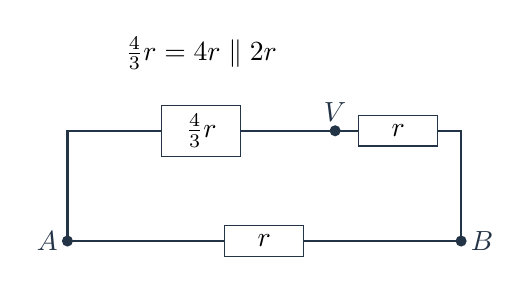
\begin{tikzpicture}
\coordinate(A)at(0,0);\coordinate(B)at(5,0);\coordinate(V)at(3.4,1.4);
\draw[body](A)--(B);
\node[draw=ink,fill=white,minimum width=10mm,minimum height=3mm]at(2.5,0){$r$};
\draw[body](A)--(0,1.4)--(V)--(5,1.4)--(B);
\node[draw=ink,fill=white,minimum width=10mm,minimum height=3mm]at(1.7,1.4){$\frac43r$};
\node[draw=ink,fill=white,minimum width=10mm,minimum height=3mm]at(4.2,1.4){$r$};
\foreach\P/\pos in{A/left,B/right,V/above}\fill[ink](\P)circle(2pt)node[\pos]{$\P$};
\node[above,align=center]at(1.7,2.05){$\frac43r=4r\parallel2r$};
\end{tikzpicture}
\end{document}
